% Shared style for all Git & GitHub lectures (same look as the N-body course)
\documentclass[11pt,a4paper]{article}
\usepackage[margin=2.3cm]{geometry}
\usepackage[T1]{fontenc}
\usepackage{lmodern}
\usepackage{upquote}   % straight quotes in monospaced text, so commands can be copied
\usepackage{microtype}
% keep '--' as two real hyphens in monospace text (commands like --version)
\DisableLigatures[-,<,>]{family=tt*}
\usepackage{booktabs,enumitem,graphicx,xcolor}
\usepackage{array}
\usepackage{needspace}
\usepackage{longtable}
\usepackage{float}
\usepackage{tikz}
\usetikzlibrary{arrows.meta,calc,positioning,decorations.pathreplacing,shapes.geometric,fit,backgrounds}
\usepackage[most]{tcolorbox}
\usepackage{listings}
\usepackage{fancyhdr}
\usepackage[colorlinks=true,linkcolor=blue!50!black,urlcolor=blue!50!black,citecolor=blue!50!black]{hyperref}

\setlength{\parindent}{0pt}
\setlength{\parskip}{0.6em}
\setlength{\abovecaptionskip}{4pt}
\usepackage[font=small,labelfont=bf]{caption}
\setlist{itemsep=0.2em,topsep=0.3em}

% ---------- colours ----------
\definecolor{cbg}{HTML}{F6F8FA}
\definecolor{ckw}{HTML}{0B5CAD}
\definecolor{ccm}{HTML}{6A737D}
\definecolor{cst}{HTML}{B5451B}
\definecolor{cpart}{HTML}{1F6FB2}
\definecolor{cheavy}{HTML}{C0392B}
\definecolor{cgreen}{HTML}{2E8B57}

% ---------- terminal listings ----------
% In a terminal session, lines starting with "$" are what YOU type.
% Everything else is what Git prints back.
\lstdefinestyle{term}{
  basicstyle=\ttfamily\small, backgroundcolor=\color{cbg},
  frame=single, rulecolor=\color{black!15}, showstringspaces=false,
  breaklines=true, columns=fullflexible, keepspaces=true,
  aboveskip=0.6em, belowskip=0.6em, xleftmargin=4pt, xrightmargin=4pt,
  literate={\$\ }{{\textcolor{cgreen}{\$\ }}}2,
  upquote=true
}
\lstset{style=term}
\newcommand{\code}[1]{\texttt{\small #1}}

% ---------- boxes ----------
\newtcolorbox{history}{colback=yellow!8,colframe=orange!60!black,
  title={History},fonttitle=\bfseries\small,left=4pt,right=4pt,top=2pt,bottom=2pt}
\newtcolorbox{quickfact}{colback=purple!4,colframe=purple!55!black,
  title={Quick fact},fonttitle=\bfseries\small,left=4pt,right=4pt,top=2pt,bottom=2pt}
\newtcolorbox{keyidea}{colback=blue!4,colframe=blue!50!black,
  title={Key idea},fonttitle=\bfseries\small,left=4pt,right=4pt,top=2pt,bottom=2pt}
\newtcolorbox{pitfall}{colback=red!4,colframe=red!55!black,
  title={Pitfall},fonttitle=\bfseries\small,left=4pt,right=4pt,top=2pt,bottom=2pt}
\newtcolorbox{tryit}{colback=teal!5,colframe=teal!55!black,
  title={Try it},fonttitle=\bfseries\small,left=4pt,right=4pt,top=2pt,bottom=2pt,breakable}
\newtcolorbox{homework}[1]{colback=green!4,colframe=green!40!black,
  title={Homework #1},fonttitle=\bfseries\small,left=4pt,right=4pt,top=2pt,bottom=2pt,
  breakable}
\newtcolorbox{goals}{colback=gray!6,colframe=gray!60!black,
  title={Learning goals},fonttitle=\bfseries\small,left=4pt,right=4pt,top=2pt,bottom=2pt}

% Solutions always start on a fresh page, behind a clear warning.
\newcommand{\solutionspage}{%
  \clearpage
  \begin{tcolorbox}[colback=red!6,colframe=red!60!black,halign=center]
    {\Large\bfseries Solutions}\\[0.3em]
    {\small Stop here if you have not tried the homework yet.\\
    Attempt every task first, run the checker, and only then read on.}
  \end{tcolorbox}
}

% ---------- Git diagram styles (TikZ) ----------
\tikzset{
  commit/.style={circle,draw=black!70,fill=blue!10,minimum size=7mm,inner sep=0pt,font=\scriptsize\ttfamily},
  newcommit/.style={commit,fill=orange!25,dashed},
  tag/.style={draw,rounded corners=2pt,font=\scriptsize\ttfamily,inner sep=2pt},
  branchtag/.style={tag,fill=green!15,draw=green!40!black},
  headtag/.style={tag,fill=yellow!30,draw=orange!70!black},
  remotetag/.style={tag,fill=purple!10,draw=purple!60!black},
  area/.style={draw,rounded corners,minimum height=11mm,minimum width=33mm,align=center,font=\small},
  cmdarrow/.style={->,thick,>=Stealth},
  link/.style={->,thick,>=Stealth,black!70},
}

% ---------- header ----------
\pagestyle{fancy}
\fancyhf{}
\renewcommand{\headrulewidth}{0.3pt}
\fancyfoot[C]{\thepage}
\newcommand{\lecturetitle}[3]{%
  \fancyhead[L]{\small\textit{Git \& GitHub from Zero}}
  \fancyhead[R]{\small Lecture #1}
  \begin{center}
    {\Large\bfseries Lecture #1}\\[0.4em]
    {\LARGE\bfseries #2}\\[0.4em]
    {\small #3}
  \end{center}
  \vspace{0.5em}
}

\begin{document}
\lecturetitle{0}{Roadmap: What Git Is, Where It Came From, and How This Course Works}{Version control, a short history, Git versus GitHub, and the order of the lectures}

\begin{goals}
\begin{itemize}
  \item Explain the problem that version control solves, in your own words.
  \item Tell apart local, centralised and distributed version control.
  \item Know the key moments in Git's history and a few quick facts about it.
  \item Explain the difference between \emph{Git} and \emph{GitHub}.
  \item Know the order of the lectures and how homework, checkers and solutions work.
\end{itemize}
\end{goals}

\section{The problem: files change, and we forget how}

Have you ever had a folder like this?

\begin{lstlisting}
report.docx
report_v2.docx
report_v2_final.docx
report_v2_final_REALLY_final.docx
report_v2_final_REALLY_final_use_this_one.docx
\end{lstlisting}

It works for a while, then it breaks down. Which file is the newest? What exactly changed between \code{v2} and \code{final}? What if a friend edits one copy while you edit another? Whose changes win? And if you delete a paragraph on Monday and need it back on Friday, where is it?

A \textbf{version control system} (VCS) solves all of these. It is a tool that
\begin{itemize}
  \item records the history of your project as a series of saved states (\emph{versions});
  \item lets you compare any two versions and go back to an old one;
  \item lets several people work at the same time and combine their work.
\end{itemize}
You keep \emph{one} folder, and the tool remembers every earlier state of it.

\begin{keyidea}
Version control is a time machine plus a collaboration tool for your files. It is used for code, but also for papers, notes, thesis chapters and configuration files: anything made of text.
\end{keyidea}

\begin{quickfact}
\textbf{Words you will meet soon} (each is explained properly later: \emph{remote} in Lecture 6, the others in Lectures 1--5). A \emph{repository} is a project folder together with its saved history. A \emph{commit} is one saved version. A \emph{branch} is a separate line of work. A \emph{remote} is a copy of the repository stored somewhere else, such as GitHub. Do not worry if these feel vague now.
\end{quickfact}

\section{Three generations of version control}

Version control tools came in three broad kinds. The diagram shows where the history of the project is stored in each.

\begin{figure}[H]
\centering
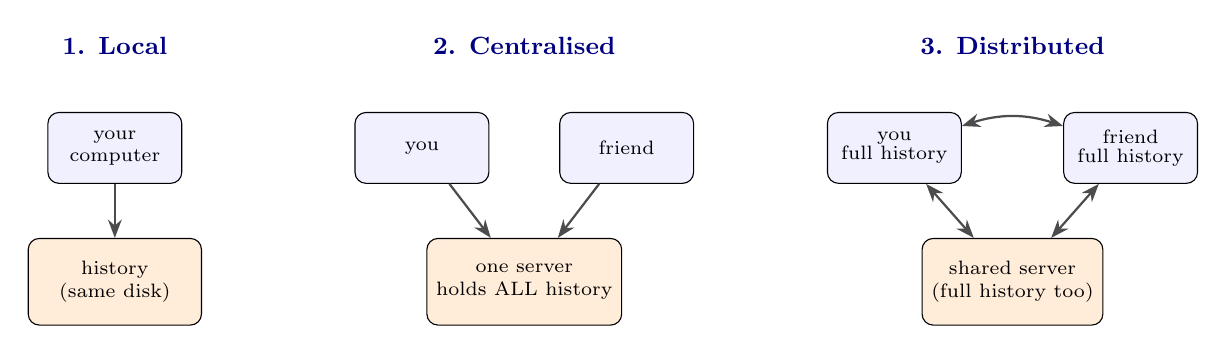
\begin{tikzpicture}[
  pc/.style={draw,rounded corners,fill=blue!6,minimum width=17mm,minimum height=9mm,font=\scriptsize,align=center},
  store/.style={draw,rounded corners,fill=orange!15,minimum width=22mm,minimum height=11mm,font=\scriptsize,align=center},
  head/.style={font=\small\bfseries,text=blue!50!black}]
  % Local
  \node[head] at (0,3.2) {1. Local};
  \node[pc] (l1) at (0,1.9) {your\\computer};
  \node[store] (ls) at (0,0.2) {history\\(same disk)};
  \draw[link] (l1)--(ls);
  % Centralised
  \node[head] at (5.2,3.2) {2. Centralised};
  \node[pc] (c1) at (3.9,1.9) {you};
  \node[pc] (c2) at (6.5,1.9) {friend};
  \node[store] (cs) at (5.2,0.2) {one server\\holds ALL history};
  \draw[link] (c1)--(cs); \draw[link] (c2)--(cs);
  % Distributed
  \node[head] at (11.4,3.2) {3. Distributed};
  \node[pc] (d1) at (9.9,1.9) {you\\[-1pt]\scriptsize full history};
  \node[pc] (d2) at (12.9,1.9) {friend\\[-1pt]\scriptsize full history};
  \node[store] (ds) at (11.4,0.2) {shared server\\(full history too)};
  \draw[link,<->] (d1)--(ds); \draw[link,<->] (d2)--(ds); \draw[link,<->] (d1) to[bend left=18] (d2);
\end{tikzpicture}
\caption{Where the history lives. In a centralised system the server is the only complete copy. In a distributed system (Git) \emph{every} computer holds the complete history. Arrows show history being copied in either direction.}
\label{fig:vcs3}
\end{figure}

\begin{description}[leftmargin=1.2em,style=nextline]
\item[Local] The history is kept on one computer (for example RCS, 1982). Simple, but no real teamwork.
\item[Centralised] One server holds the history; you download a working copy of the files and send changes back (for example CVS, Subversion). Teamwork is possible, but if the server is down or you have no internet, you cannot save history or look at old versions.
\item[Distributed] Everyone has a full copy of the whole history (Git, Mercurial). You can work offline, save versions as often as you like, and copy history to or from any other computer, with or without a server. A shared server is still useful, but it is a convenience, not a requirement.
\end{description}

\section{A short history of Git}

This section is background. Read it for context; you will not be tested on dates.

\begin{history}
Git was created in \textbf{April 2005} by Linus Torvalds, the creator of Linux. The Linux kernel team had been using a proprietary distributed tool called BitKeeper. When the free-use arrangement ended, the team needed a replacement. Torvalds wanted something fast, distributed, and safe against accidental corruption, and no existing free tool fit. He started writing Git on 3 April 2005. Within days Git could manage its own source code, and the kernel started using it that month. A few months later, Junio Hamano took over as maintainer, a role he still holds.
\end{history}

\begin{center}{\small
\begin{tabular}{@{}r p{11.5cm}@{}}
\toprule
Year & Milestone \\
\midrule
1972 & SCCS: one of the first version-control tools (Bell Labs). \\
2000 & Subversion (SVN) development starts (1.0 in 2004): a better centralised system, widely used for years. \\
2005 & Git (Torvalds) and Mercurial appear within weeks of each other, both distributed. \\
2008 & GitHub launches: a website for hosting Git repositories with tools for teamwork. \\
2018 & Microsoft announces it will buy GitHub (the purchase completes the same year). \\
2020 & New repositories on GitHub start on a branch called \code{main} instead of \code{master}; Git 2.28 lets you choose this name yourself (you do so in Homework 0). \\
\bottomrule
\end{tabular}}\end{center}

\begin{quickfact}
\begin{itemize}
  \item Git is free, open source, and works on Linux, macOS and Windows. The word ``git'' is British slang for an unpleasant person; Torvalds joked that he names his projects after himself.
  \item Every saved version in Git gets a unique ID: a 40-character code (by default) called a \emph{hash}, such as \code{3f2a9c1\dots}. You will usually need only the first 7 characters (Lecture 3 shows where to see them).
\end{itemize}
\end{quickfact}

\section{Git is not GitHub}

This is the most common confusion for beginners.

\begin{figure}[H]
\centering
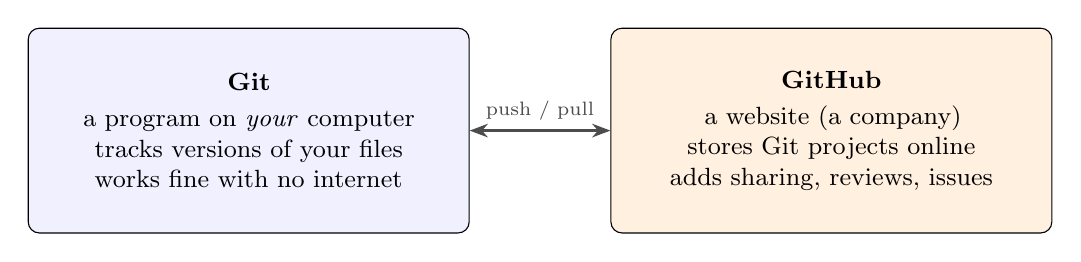
\begin{tikzpicture}[
  big/.style={draw,rounded corners,minimum width=5.6cm,minimum height=2.6cm,align=center,text width=5.2cm,font=\small}]
  \node[big,fill=blue!6] (git) at (0,0) {\textbf{Git}\\[2pt]a program on \emph{your} computer\\tracks versions of your files\\works fine with no internet};
  \node[big,fill=orange!12] (gh) at (7.4,0) {\textbf{GitHub}\\[2pt]a website (a company)\\stores Git projects online\\adds sharing, reviews, issues};
  \draw[link,<->] (git) -- node[above,font=\scriptsize] {push / pull} (gh);
\end{tikzpicture}
\caption{Git does the version tracking. GitHub is one place to keep a copy online and collaborate. Other sites (GitLab, Bitbucket, Codeberg) do a similar job.}
\end{figure}

An analogy: Git is like a very powerful ``version history'' feature, but for a whole folder, and it lives on your own computer. GitHub is like a shared cloud folder that stores that history online and lets friends comment on it. You can use Git without GitHub, but you cannot use GitHub's sharing without Git. In this course you learn Git first (Lectures 1--5), because GitHub's sharing features are built on top of it.

\Needspace{26\baselineskip}
\section{The order of the course}

The order below rises in difficulty. \textbf{Each lecture reuses what you learned in the previous one.}

\begin{figure}[H]
\centering
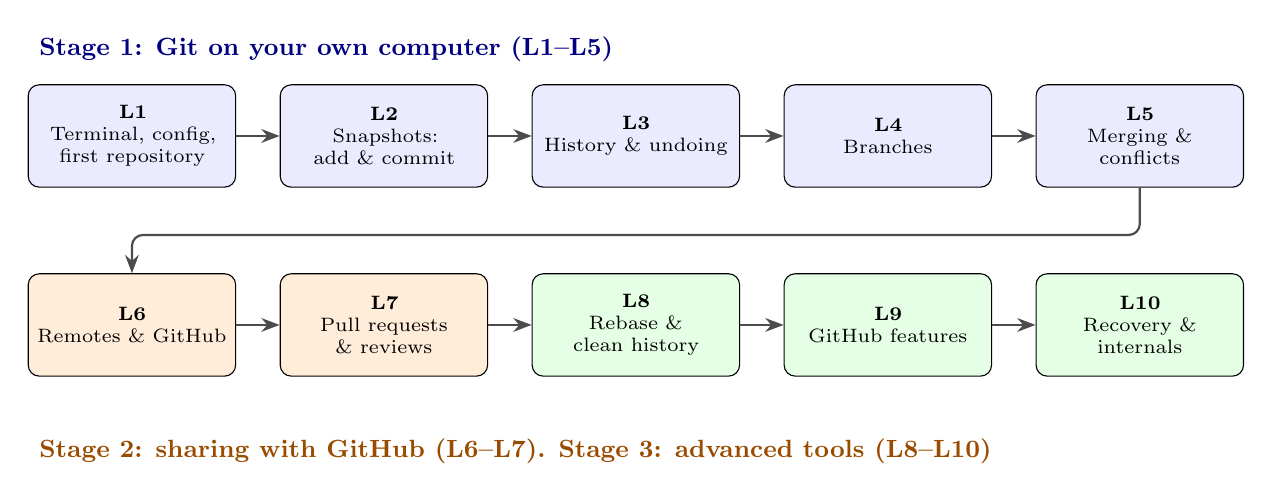
\begin{tikzpicture}[
  lec/.style={draw,rounded corners,minimum width=26mm,minimum height=13mm,align=center,font=\scriptsize,text width=24mm},
  g/.style={lec,fill=blue!8}, h/.style={lec,fill=orange!15}, a/.style={lec,fill=green!10}]
  \node[g] (l1) at (0,0)    {\textbf{L1}\\Terminal, config, first repository};
  \node[g] (l2) at (3.2,0)  {\textbf{L2}\\Snapshots: add \& commit};
  \node[g] (l3) at (6.4,0)  {\textbf{L3}\\History \& undoing};
  \node[g] (l4) at (9.6,0)  {\textbf{L4}\\Branches};
  \node[g] (l5) at (12.8,0) {\textbf{L5}\\Merging \& conflicts};
  \node[h] (l6) at (0,-2.4)    {\textbf{L6}\\Remotes \& GitHub};
  \node[h] (l7) at (3.2,-2.4)  {\textbf{L7}\\Pull requests \& reviews};
  \node[a] (l8) at (6.4,-2.4)  {\textbf{L8}\\Rebase \& clean history};
  \node[a] (l9) at (9.6,-2.4)  {\textbf{L9}\\GitHub features};
  \node[a] (l10) at (12.8,-2.4) {\textbf{L10}\\Recovery \& internals};
  \draw[link] (l1)--(l2); \draw[link] (l2)--(l3); \draw[link] (l3)--(l4); \draw[link] (l4)--(l5);
  \draw[link,rounded corners] (l5.south) -- ++(0,-0.6) -| (l6.north);
  \draw[link] (l6)--(l7); \draw[link] (l7)--(l8); \draw[link] (l8)--(l9); \draw[link] (l9)--(l10);
  \node[font=\small\bfseries,text=blue!50!black,anchor=west] at (-1.3,1.1) {Stage 1: Git on your own computer (L1--L5)};
  \node[font=\small\bfseries,text=orange!60!black,anchor=west] at (-1.3,-4.0) {Stage 2: sharing with GitHub (L6--L7). Stage 3: advanced tools (L8--L10)};
\end{tikzpicture}
\caption{Course map. Blue (L1--5): Git on one computer. Orange (L6--7): sharing and teamwork. Green (L8--10): advanced tools. Follow the arrows.}
\end{figure}

\begin{center}
\small\renewcommand{\arraystretch}{1.15}
\begin{tabular}{@{}c >{\raggedright\arraybackslash}p{4.4cm} >{\raggedright\arraybackslash}p{8.2cm}@{}}
\toprule
\# & Lecture & What you can do afterwards \\
\midrule
1 & First steps & Use the terminal; configure Git; turn a folder into a repository \\
2 & Snapshots & Save versions with \code{add} and \code{commit}; ignore files \\
3 & History \& undoing & Read the history; compare versions; undo mistakes safely \\
4 & Branches & Work on an idea separately without breaking the main line \\
5 & Merging \& conflicts & Combine branches; resolve a conflict calmly \\
6 & Remotes \& GitHub & Put your project on GitHub; \code{clone}, \code{push}, \code{pull} \\
7 & Pull requests \& reviews & Contribute to a friend's project; review each other's work \\
8 & Rebase \& cherry-pick & Tidy up history; cherry-pick; push rewritten history safely \\
9 & GitHub features & Issues, Actions (automated checks), branch protection, releases \\
10 & Recovery \& internals & Rescue lost work (reflog, \code{reset}, \code{stash}, \code{bisect}); look inside \code{.git} \\
\bottomrule
\end{tabular}
\end{center}

\textbf{Why this order?} GitHub's sharing is Git with a website on top, so we first learn Git alone (L1--5), where mistakes cannot affect anyone else. We first learn how a single copy of a project works. Rebase and recovery come last because they are most useful once you understand the simpler tools they replace or repair.

\textbf{What you need.} No programming experience. A computer, a text editor (any will do, even Notepad or TextEdit in plain-text mode), a terminal (a text window where you type commands instead of clicking), and a free GitHub account (needed from Lecture~6). Plan one to two hours per lecture.

\section{How the homework works}

\begin{keyidea}
Type every command yourself. Reading about Git is not enough: your hands need to learn it too. Mistakes in a practice repository cost nothing.
\end{keyidea}

\Needspace{8\baselineskip}
Each lecture ends with a \textbf{Homework} box with tasks. You will do the work in the terminal. Most lectures come with three helpers:

\begin{enumerate}
  \item \textbf{A setup script}, \code{codeHints/Lxx/setup\_hwX.sh}, which builds a practice repository in the \code{practice/} folder, already in the starting state for the tasks.
  \item \textbf{A checker}, \code{codeHints/Lxx/check\_hwX.sh}, which looks at your repository and prints \code{PASS} or \code{FAIL} for each task (\code{SKIP} for an optional check that could not run).
  \item \textbf{Solutions}, in two places: at the end of every lecture PDF, always starting on a new page, and as a separate PDF in \code{solutions/Lxx/}.
\end{enumerate}
Some lectures also have a follow-along repository (\code{setup\_demoN.sh}) and, from Lecture 6, a ``friend'' script that plays a teammate.

Here \code{Lxx} stands for a lecture folder such as \code{L02}, and \code{hwX} for its homework number. The course folder looks like this:
\begin{lstlisting}
LearningGit/
  lectures/     the PDFs
  codeHints/    setup and check scripts for each lecture
  solutions/    solution PDFs
  practice/     your sandbox repositories (created by the setup scripts)
\end{lstlisting}
The workflow is: read the lecture, run the setup script, do the tasks, run the checker until everything says \code{PASS}, and \emph{only then} open the solutions to compare your approach with the reference.

Always start in the course folder \code{LearningGit/}. (\code{cd} means ``change directory''; Lecture~1 explains it.) Here is an \emph{illustration} from Lecture~2; do not run it yet:
\begin{lstlisting}
$ bash codeHints/L02/setup_hw2.sh     # build the practice repository
$ cd practice/hw2                     # go into it and do the tasks
$ cd ../..                            # back to the course folder
$ bash codeHints/L02/check_hw2.sh
PASS  setup: practice/hw2 is its own repository
FAIL  2.1/2.2/2.3 exactly three commits
\end{lstlisting}

If a check says \code{FAIL}, fix your repository and run the checker again.

In terminal listings, a line that starts with \code{\$} is what \emph{you} type (do not type the \code{\$} itself). Other lines are what the computer prints. Text after \code{\#} is a comment.

\textbf{Note for Windows and macOS.} The scripts run with the \code{bash} command. On Windows, use \emph{Git Bash} (installed with Git for Windows). On macOS, \code{bash script.sh} works even though the default shell is \code{zsh}.

\section{Homework 0}

\begin{homework}{0: Get ready}
You need a terminal and Git installed. A \emph{terminal} is a window where you type commands. Open it as follows (Lecture~1 teaches the basics):
\begin{itemize}
  \item \textbf{macOS:} open the app \emph{Terminal} (Spotlight search). Typing \code{git --version} offers to install Git if it is missing.
  \item \textbf{Windows:} install Git from \url{https://git-scm.com/downloads}, then open \emph{Git Bash} from the Start menu.
  \item \textbf{Linux:} open your terminal and install Git with your package manager, for example \code{sudo apt install git}.
\end{itemize}

\begin{description}[leftmargin=1.2em,style=nextline]
\item[0.1 Install] Install Git if needed (on Windows, open Git Bash only after installing), then run \code{git --version} in the terminal. It should print a version, such as \code{git version 2.43.0}. You need version 2.28 or newer (older versions do not support the setting in 0.3; if yours is older, update from \url{https://git-scm.com/downloads}).
\item[0.2 Introduce yourself] Tell Git who you are. Every saved version records its author. Keep the quotation marks and replace the placeholder text with your own:
\begin{lstlisting}
$ git config --global user.name "Your Name"
$ git config --global user.email "you@example.com"
\end{lstlisting}
Use the same email you use (or will use) on GitHub.
\item[0.3 Default branch name] Set the name of the first branch of new repositories to \code{main}. (A branch is a line of saved versions; you meet it in Lecture~4, so for now just copy the command.)
\begin{lstlisting}
$ git config --global init.defaultBranch main
\end{lstlisting}
\item[0.4 Short answer] In two or three sentences, explain the difference between Git and GitHub, as if to a friend who has never heard of either.
\item[0.5 GitHub account] Create a free account at \url{https://github.com} (needed from Lecture~6).
\item[0.6 Thinking] Name a time you wished you had version control.
\end{description}
\textbf{Check yourself:} run \code{bash codeHints/L00/check\_hw0.sh} from the course folder (\code{LearningGit/}). It checks tasks 0.1--0.3. Tasks 0.4--0.6 you compare with the solutions.
\end{homework}

\section{Summary}

\begin{itemize}
  \item Version control records a project's history so you can compare, go back and collaborate. Git (Torvalds, 2005) is distributed: every copy holds the full history. Git is the tool on your computer; GitHub is a website that hosts Git projects.
  \item The course goes from Git on your own computer (L1--5) to sharing (L6--7) to advanced tools (L8--10). Further reading: \emph{Pro Git}, free at \url{https://git-scm.com/book}, Chapter 1.
\end{itemize}

\solutionspage

\section*{Solutions to Homework 0}

\textbf{0.1.} \code{git --version} prints something like \code{git version 2.43.0}. If you get ``command not found'', Git is not installed, or the terminal needs to be reopened after installing.

\textbf{0.2.} After running the two commands, check them with
\begin{lstlisting}
$ git config --global user.name
Your Name
$ git config --global user.email
you@example.com
\end{lstlisting}
(Your own name and email will appear. \code{git config --global --list} shows all your settings.)

\textbf{0.3.} Check with \code{git config --global init.defaultBranch}. It should print \code{main}.

\textbf{0.4.} Model answer: ``Git is a program on your computer that remembers every saved version of your files and lets you go back or combine work. GitHub is a website where you can store a copy of a Git project online to share it and work with others. You can use Git without GitHub, but not GitHub without Git.''

\textbf{0.5.} Sign-up is checked by logging in at github.com. Nothing else to submit.

\textbf{0.6.} Any honest example is correct. Typical ones: a report or thesis where an old paragraph was deleted and needed again; two people editing different copies of the same file; ``it worked yesterday, what did I change?''



\end{document}
